\documentclass[12pt,halfline,a4paper]{ouparticle}

\begin{document}

\title{Ball Sinking into a Viscous Fluid} 

\author{%
\name{Li Ruixiang}
\email{\texttt{liruixiang@zju.edu.cn}}
}
\date{}

\maketitle
\tableofcontents
\newpage

\section{Motion of a Ball Sinking into a Viscous Fluid}
一个刚体在液体中的运动由下列的运动方程描述:
\begin{equation}\begin{aligned}
    & \rho_{p}V_{c}\dot{\boldsymbol{u}}_{c}=\rho_{f}\oint_{\partial S}\boldsymbol{\tau}\cdot\boldsymbol{n}\mathrm{d}\sigma+(\rho_{p}-\rho_{f})V_{c}\boldsymbol{g}, \\
    & I_{c}\dot{\boldsymbol{\omega}}_{c}=\rho_{f}\oint_{\partial S}\boldsymbol{r}\times(\boldsymbol{\tau}\cdot\boldsymbol{n})\mathrm{d}\sigma,
   \end{aligned}\end{equation}
其中$\rho_{p}$是刚体的密度,$V_{c}$是刚体的体积,$\boldsymbol{u}_{c}$是刚体的质心速度,$\rho_{f}$是流体的密度,$\boldsymbol{\tau}$是应力张量,$\boldsymbol{n}$是单位法向量,$\boldsymbol{g}$是重力加速度,$I_{c}$是刚体的转动惯量,$\boldsymbol{\omega}_{c}$是刚体的角速度,$\boldsymbol{r}$是刚体上的点到质心的矢量,$S$是刚体的表面.
对于不可压流体,应力张量$\boldsymbol{\tau}$可以表示为
$$\boldsymbol \tau = -pI + \nu (\nabla \boldsymbol{u} + (\nabla \boldsymbol{u})^T)$$

\section{Coupling of the Solid and the Fluid}
固液边界的耦合条件为无滑移边界条件,即液体和固体之间的相对速度为0.
固体的速度可以表示为平动和转动的合成:
\begin{equation}\boldsymbol u(\boldsymbol{x})=\boldsymbol{u}_c+\boldsymbol{\omega}_c\times(\boldsymbol{x}-\boldsymbol{x_c}),\end{equation}

\section{Processing CutCell}
按照Cell-Liniking method\cite{celllinking,stateredistribution}的思路,对于这些CutCell,首先需要计算出处于液体区域的体积和质心,然后考虑在质心处的多重Taylor展开,通过最小二乘法来计算展开式的系数\cite{fourthorder}.


\subsection{Volume and Centroid Calculation}
在计算时,为了不失一般性,我们选择根据CutCell的不同情况,选择合适的cell顶点来构建一个曲边三角形\cite{NEFEM},并通过映射将其映射到参考单元上,然后计算参考单元上的积分.

\begin{equation}
    \begin{aligned}
        \boldsymbol{\psi} : R=[ \lambda_{1}^{e}, \lambda_{2}^{e} ] \times[ 0, 1 ] &\longrightarrow\Omega_{e} \\
        \boldsymbol{\lambda}=( \lambda, \vartheta) &\longmapsto\boldsymbol{\psi} ( \boldsymbol{\lambda} ) :=\boldsymbol{C} ( \lambda) ( 1-\vartheta)+\vartheta\boldsymbol{x}_{3}, \\
    \end{aligned}
\end{equation}
\begin{figure}[h]
    \centering  

    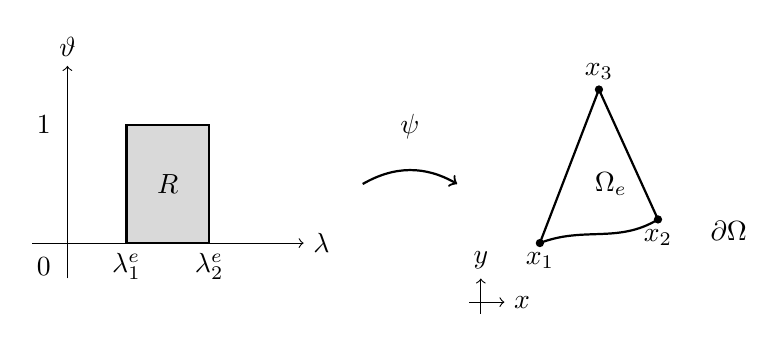
\begin{tikzpicture}[scale=1.5]

    % 左侧图形 - 阴影区域从 lambda_1 到 lambda_2
    \fill[gray!30] (0.5,0) rectangle (1.2,1); % 调整阴影的起点到 lambda_1
    \draw[thick] (0.5,0) rectangle (1.2,1);
    
    % 左侧坐标轴
    \draw[->] (-0.3,0) -- (2.0,0) node[right] {$\lambda$};
    \draw[->] (0,-0.3) -- (0,1.5) node[above] {$\vartheta$};
    
    % 左侧坐标标签
    \node at (0.5,-0.2) {$\lambda_1^e$}; % lambda_1^e 位置右移
    \node at (1.2,-0.2) {$\lambda_2^e$};
    \node at (-0.2,1) {$1$};
    \node at (-0.2,-0.2) {$0$};
    
    % 矩形内部标记
    \node at (0.85,0.5) {$R$}; % 调整标签位置
    
    % 映射箭头

    \draw[->, thick, bend left] (2.5,0.5) to (3.3,0.5);
    \node[above] at (2.9,0.8) {$\boldsymbol{\psi}$};
    \draw[thick] (4,0) -- (4.5,1.3);
    \draw[thick] (4.5,1.3) -- (5,0.2);
     % 在 x1 和 x2 之间画一条弯曲的线
    \draw[thick, bend left] (4,0) to[out=10, in=200] (5,0.2);
    
    % % 三角形顶点标记
    \fill (4,0) circle (1pt) node[below] {$x_1$};
    \fill (5,0.2) circle (1pt) node[below] {$x_2$};
    \fill (4.5,1.3) circle (1pt) node[above] {$x_3$};
    
  
    \node at (4.6,0.5) {$\Omega_e$}; % 调整标签位置
    \node at (5.6,0.1) {$\partial\Omega$};

    \draw[->] (3.4,-0.5) -- (3.7,-0.5) node[right] {$x$};
    \draw[->] (3.5,-0.6) -- (3.5,-0.3) node[above] {$y$};
    \end{tikzpicture}

    \caption{Mapping of the reference element $R$ to the physical element $\Omega_e$}
    \label{fig:mapping}
\end{figure}
\newline 
于是,体积和质心的计算可以表示为:
\begin{equation}\label{eq:volume_centorid}
\begin{aligned}
    V_{c} &= \int_{R} |J_{\boldsymbol{\psi}}(\boldsymbol{\lambda})| \mathrm{d} \boldsymbol{\lambda}\\
    \boldsymbol{x}_{c} &= \frac{1}{V_{c}} \int_{R} \boldsymbol{\psi}(\boldsymbol{\lambda}) |J_{\boldsymbol{\psi}}(\boldsymbol{\lambda})|\boldsymbol{\lambda}
\end{aligned}
\end{equation}
以上的计算采用$R$上的Gauss-Legendre型积分公式.

\subsection{Cell Division}
根据cell与边界曲线的位置关系,将其分为不同的类别.
\begin{figure}[h]
    \centering
    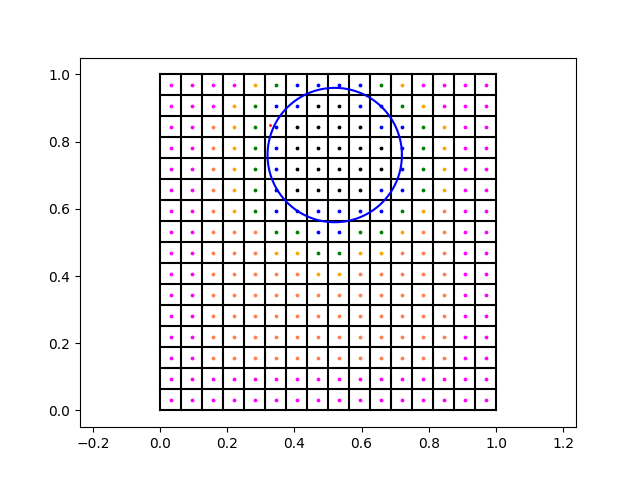
\includegraphics{figure/cycle.png}
    \caption{Cell Division}
    \label{fig:cell_division}
\end{figure}


\subsection{Diffculties in the specific case}
在大多数情况下,边界曲线与Cell只会切出一个部分,但是在某些特殊情况下,边界曲线会切出两个部分,如图\ref{fig:cut_cell_example}所示,阴影部分表示固体区域,在图中以虚线标记计算单元,实线表示边界曲线,蓝色实心点表示边界和单元的交点,可以看到边界曲线切出了两个部分.



\begin{figure}[h]
    \centering
    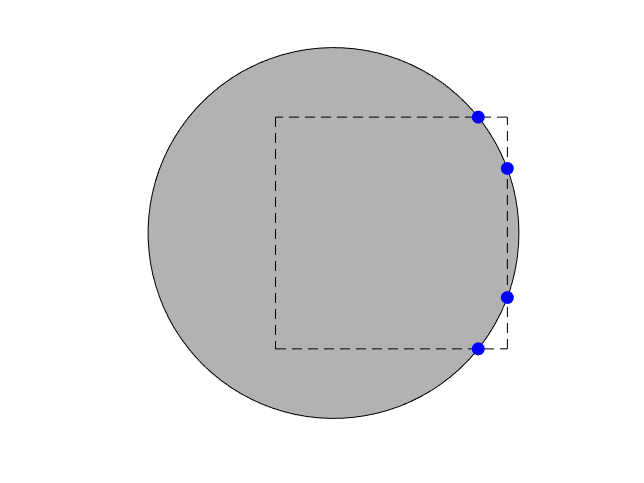
\includegraphics[width=0.5\textwidth]{figure/cut_cell_example.png}
    \caption{Example: A cell is cut by the curve twice.}
    \label{fig:cut_cell_example}
\end{figure}






\newpage
\bibliographystyle{plain}
\bibliography{ref}


\end{document}